\documentclass[11pt, a4paper]{article}

% --- Packages ---
\usepackage[utf8]{inputenc}
\usepackage[margin=1in, top=0.6in]{geometry} 
\usepackage{titlesec}
\usepackage{enumitem}
\usepackage{hyperref}
\usepackage{amsmath, amssymb}
\usepackage{listings}
\usepackage{xcolor}
\usepackage{titling}
\usepackage{graphicx}
\usepackage{booktabs}
\usepackage{float}
\usepackage{tikz}
\usetikzlibrary{shapes.geometric, arrows.meta, positioning}

% --- Title Adjustment ---
\setlength{\droptitle}{-4em} 
\date{\vspace{-4em}}

% --- Document Info ---
\title{\textbf{Assignment 2 Report}}
\author{Hsu Shu Wei 112550191}

\begin{document}

\maketitle

\noindent
\textbf{GitHub Repository}: \url{https://github.com/mikehsuhoodie/DM2026-Assignment-2}

\section*{1. K-fold Cross-Validation}
\subsection*{(a) 5-fold cross-validation average accuracy on the training data}

The table below shows the 5-fold cross-validation average accuracy on the training data for different combinations of learning rates and regularization parameters (\texttt{reg\_lambda}).

\begin{table}[H]
    \centering
    \begin{tabular}{@{}lcccc@{}}
        \toprule
        \textbf{Learning Rate} & \textbf{$\lambda = 1.0$} & \textbf{$\lambda = 2.0$} & \textbf{$\lambda = 4.0$} & \textbf{$\lambda = 8.0$} \\ \midrule
        \textbf{0.005}         & 0.7171                 & 0.7200                 & 0.7257                 & 0.7229                 \\
        \textbf{0.010}         & 0.7229                 & 0.7286                 & 0.7257                 & 0.7171                 \\
        \textbf{0.100}         & 0.7229                 & 0.7257                 & 0.7257                 & 0.7171                 \\
        \textbf{0.500}         & 0.7229                 & 0.6914                 & 0.5343                 & 0.4657                 \\ \bottomrule
    \end{tabular}
    \caption{5-fold CV accuracy across different hyperparameters.}
\end{table}

\subsection*{(b) Top Two Hyperparameter Settings}

The top two settings selected based on the highest average cross-validation accuracy on the training data are:
\begin{itemize}
    \item \textbf{Top 1:} \texttt{learning\_rate} = 0.01, \texttt{reg\_lambda} = 2.0 (Mean Accuracy: 0.7286, Std: 0.0579)
    \item \textbf{Top 2:} \texttt{learning\_rate} = 0.005, \texttt{reg\_lambda} = 4.0 (Mean Accuracy: 0.7257, Std: 0.0331)
\end{itemize}

Testing results for Top 1: Accuracy = 0.7600, Precision = 0.7381, Recall = 0.8158, F1-score = 0.7750.\\
Testing results for Top 2: Accuracy = 0.7533, Precision = 0.7241, Recall = 0.8289, F1-score = 0.7730.

\begin{figure}[H]
    \centering
    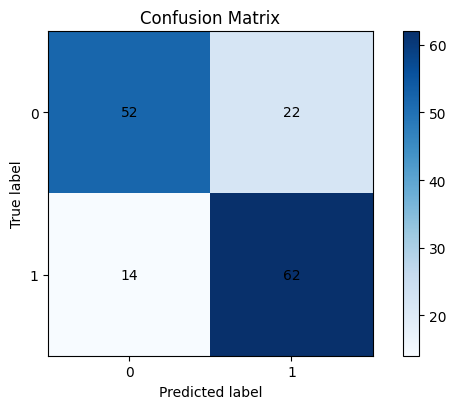
\includegraphics[width=0.45\textwidth]{pics/section1-1.png}
    \hfill
    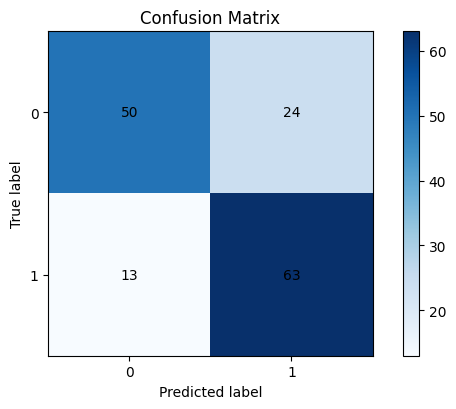
\includegraphics[width=0.45\textwidth]{pics/section1-2.png}
    \caption{Testing Results for Top 1 (left) and Top 2 (right).}
\end{figure}

\subsection*{(c) Observations}
\begin{enumerate}
    \item The best settings are close to each other, which suggests that the model is not extremely sensitive to small changes in learning rate or regularization in this range.
    \item Very large learning rate with strong regularization becomes unstable, especially when \texttt{learning\_rate}=0.5 and \texttt{reg\_lambda} is large. This likely makes the gradient updates too aggressive and prevents the model from settling into a good decision boundary.
    \item The selected top two settings perform similarly on the test set, so the cross-validation result is reasonably consistent with unseen data instead of being only a training-split accident.
    \item When two settings have nearly the same accuracy, I would prefer the one with smaller fold-to-fold variation because it is less dependent on a lucky split.
\end{enumerate}


\section*{2. SVM}
\subsection*{(a) SVM with C=1.0}
\begin{table}[H]
    \centering
    \begin{tabular}{@{}lcc@{}}
        \toprule
        \textbf{Split} & \textbf{Accuracy} & \textbf{Weighted F1-score} \\ \midrule
        Training       & 0.9808            & 0.9809                     \\
        Validation     & 0.8625            & 0.8630                     \\
        Test           & 0.8975            & 0.8979                     \\ \bottomrule
    \end{tabular}
    \caption{Performance of SVM with C=1.0.}
\end{table}

\subsection*{(b) Exploration of Different C Values}
\begin{figure}[H]
    \centering
    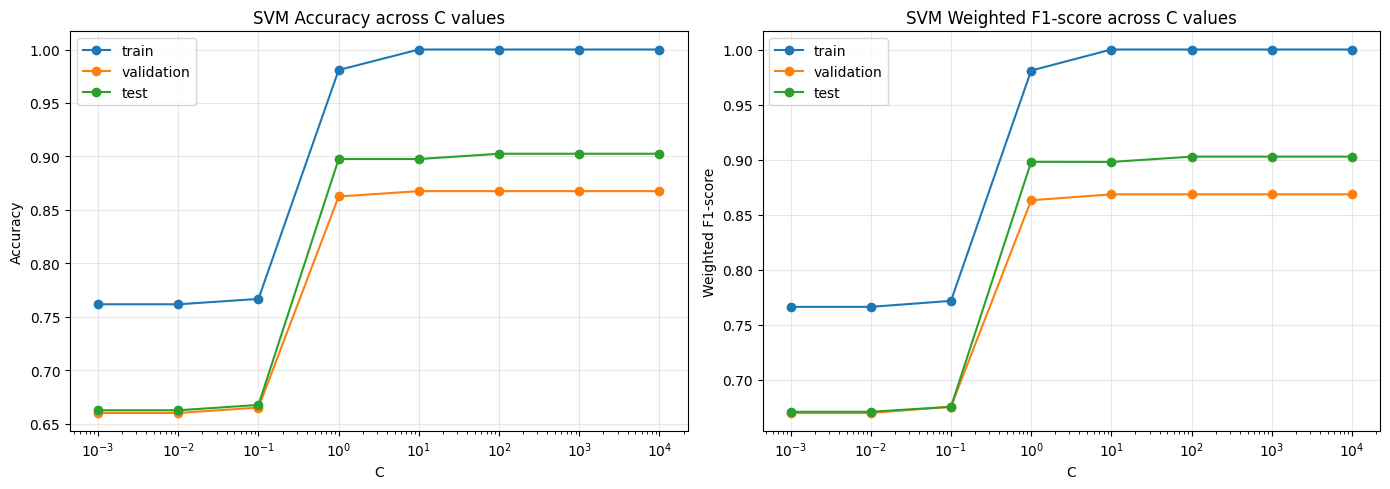
\includegraphics[width=0.85\textwidth]{pics/section2-1.png}
    \caption{SVM performance across different values of C.}
\end{figure}

\subsection*{(c) Generalization Observation}
The SVM shows the usual regularization trade-off. A very small $C$ makes the classifier too conservative, so it cannot fit enough of the class boundary. Increasing $C$ improves validation performance at first, but after a point the gain becomes small because the model is already flexible enough. I choose $C=10$ because it gives the best validation behavior without relying only on the almost-perfect training score, which would be a weaker sign of generalization.

\section*{3. Association Rule Mining}
\subsection*{(a) Frequent Patterns}
All frequent patterns showing support $\geq$ 0.3 using FP-growth:
\begin{table}[H]
    \centering
    \begin{tabular}{@{}lc@{}}
        \toprule
        \textbf{Itemset} & \textbf{Support} \\ \midrule
        \texttt{ram\_medium} & 0.6820 \\
        \texttt{px\_width\_medium} & 0.4160 \\
        \texttt{battery\_power\_medium} & 0.4140 \\
        \texttt{int\_memory\_medium} & 0.4120 \\
        \texttt{battery\_power\_medium, ram\_medium} & 0.3180 \\
        \texttt{int\_memory\_low} & 0.3160 \\
        \texttt{battery\_power\_low} & 0.3080 \\
        \texttt{px\_width\_medium, ram\_medium} & 0.3060 \\ \bottomrule
    \end{tabular}
    \caption{Frequent patterns with support $\geq$ 0.3.}
\end{table}

\subsection*{(b) Association Rules}
Association rules where support $\geq$ 0.3, confidence $\geq$ 0.4 and lift $\geq$ 0.8:
\begin{table}[H]
    \centering
    \resizebox{\textwidth}{!}{
    \begin{tabular}{@{}llccc@{}}
        \toprule
        \textbf{Antecedents} & \textbf{Consequents} & \textbf{Support} & \textbf{Confidence} & \textbf{Lift} \\ \midrule
        \texttt{battery\_power\_medium} & \texttt{ram\_medium}           & 0.3180 & 0.7681 & 1.1263 \\
        \texttt{ram\_medium}           & \texttt{battery\_power\_medium} & 0.3180 & 0.4663 & 1.1263 \\
        \texttt{px\_width\_medium}     & \texttt{ram\_medium}           & 0.3060 & 0.7356 & 1.0786 \\
        \texttt{ram\_medium}           & \texttt{px\_width\_medium}     & 0.3060 & 0.4487 & 1.0786 \\ \bottomrule
    \end{tabular}}
    \caption{Association rules meeting the specified criteria.}
\end{table}

\subsection*{(c) Observations}
\begin{enumerate}
    \item Most frequent patterns for \texttt{price\_range=1} are medium-level hardware specifications. This matches the intuition that this class represents mid-range phones rather than extremely cheap or premium phones.
    \item \texttt{ram\_medium} appears in several frequent itemsets, so RAM seems to be a central attribute for describing this price group.
    \item The association between medium battery power and medium RAM is meaningful because these two features appear together more often than random independence would suggest. In practice, manufacturers may balance memory and battery capacity for mid-range devices.
    \item The rules are useful as descriptive patterns, but they should not be interpreted as causal relationships. They show co-occurrence inside this subset of data, not that one feature directly determines another.
\end{enumerate}

\section*{4. PCA and K-Means}
\subsection*{(a) Feature Standardization}
The dataset \texttt{mobile\_price.csv} was split into features $X$ and labels $y$ (\texttt{price\_range}). All features were standardized using z-score normalization via \texttt{sklearn.preprocessing.StandardScaler}, resulting in zero mean and unit variance for each feature.

\subsection*{(b) PCA Projection to 2 Dimensions}
The standardized features were projected onto 2 principal components using PCA. PC1 explains 0.0839 and PC2 explains 0.0811 of the total variance, for a combined total of 0.1650 (16.5\%).

\begin{figure}[H]
    \centering
    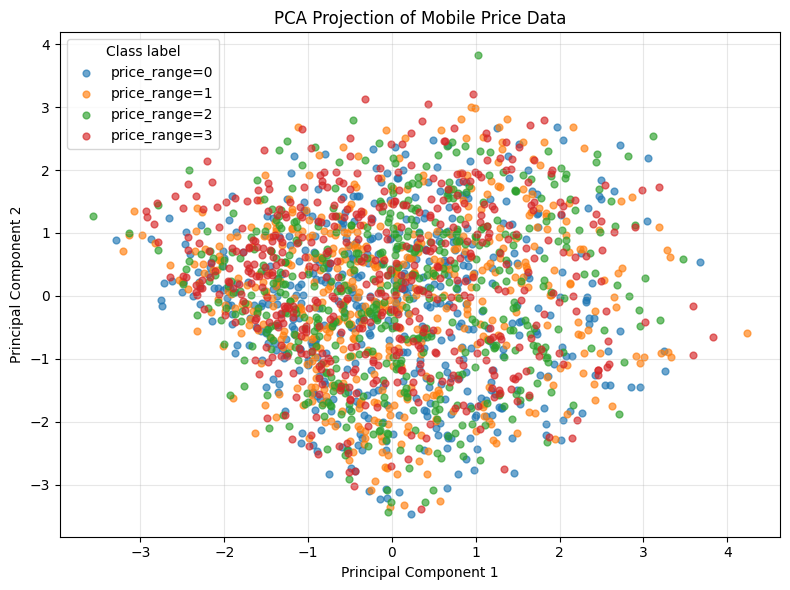
\includegraphics[width=0.6\textwidth]{pics/section4-1.png}
    \caption{PCA projection of features onto 2 dimensions, colored by price range label.}
\end{figure}

\subsection*{(c) K-means Clustering (All Features)}
K-means with $k=4$ was applied to all standardized features. The clustering was evaluated against the true price-range labels using the Adjusted Rand Index (ARI = 0.0060).

\begin{figure}[H]
    \centering
    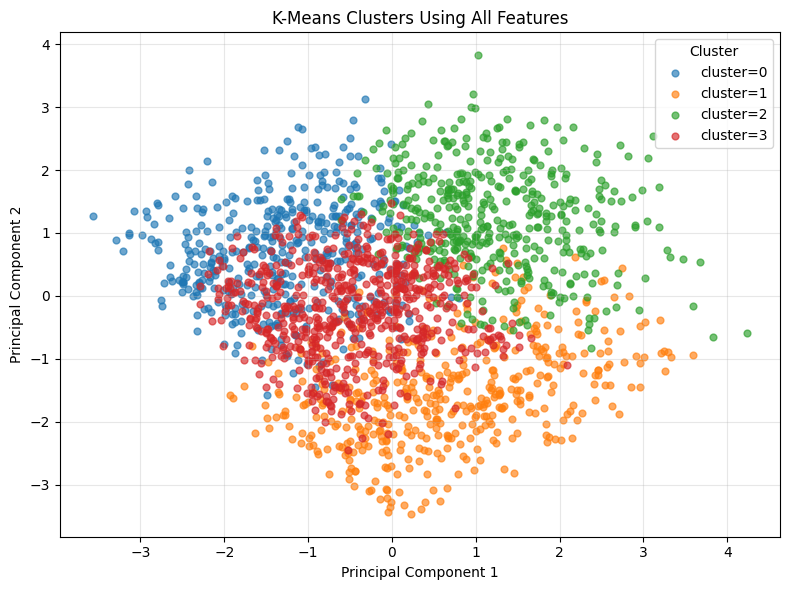
\includegraphics[width=0.6\textwidth]{pics/section4-2.png}
    \caption{K-means clustering using all standardized features.}
\end{figure}

\subsection*{(d) K-means Clustering (PCA 2D Features)}
K-means with $k=4$ was applied to the 2-dimensional PCA features from 4(b). The clustering performance was ARI = 0.0017.

\begin{figure}[H]
    \centering
    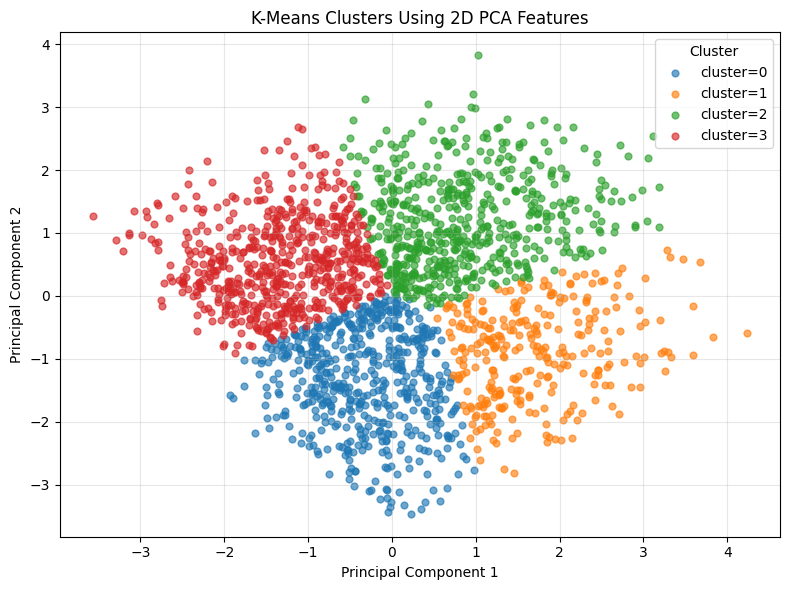
\includegraphics[width=0.6\textwidth]{pics/section4-3.png}
    \caption{K-means clustering using 2-dimensional PCA features.}
\end{figure}

\subsection*{(e) Observations}
\begin{enumerate}
    \item The PCA scatter plot is easy to visualize, but the first two components keep only a small part of the total information. Therefore, overlapping points in the plot do not necessarily mean the classes are completely inseparable in the full feature space.
    \item K-means does not align well with \texttt{price\_range}, which suggests that the price classes are not naturally shaped as compact spherical clusters.
    \item Using all standardized features is still slightly better than clustering on only two PCA dimensions, so some useful signal is lost when the data is compressed too aggressively for visualization.
    \item This result shows a limitation of unsupervised clustering for this dataset: the labels are based on price category, but K-means only sees geometric distance and has no direct knowledge of which features matter most for price.
\end{enumerate}

\section*{5. Enhancing K-means Clustering with Association Rule Mining}

% ---- Framework Diagram ----
\subsection*{Framework Diagram}

\begin{figure}[H]
\centering
\begin{tikzpicture}[
    box/.style={rectangle, draw, rounded corners=4pt,
                minimum width=7cm, minimum height=0.65cm,
                text centered, font=\small,
                fill=blue!8, draw=blue!40!black},
    arrow/.style={-Stealth, thick, blue!60!black},
    node distance=0.45cm
]
\node[box] (raw)      {Raw Mobile Dataset};
\node[box] (disc)     [below=of raw]      {Feature Discretization \quad (low / medium / high bins)};
\node[box] (label)    [below=of disc]     {Append \texttt{price\_range\_k} to each transaction};
\node[box] (arm)      [below=of label]    {FP-growth Association Rule Mining};
\node[box] (filter)   [below=of arm]      {Rule Filtering: consequent contains \texttt{price\_range\_k}, lift $>$ 1};
\node[box] (weight)   [below=of filter]   {Feature Weight: $w_f = \sum_{\text{rules}} \text{supp} \times \text{conf} \times \text{lift}$};
\node[box] (weighted) [below=of weight]   {Multiply Standardized Features by $w_f$};
\node[box] (kmeans)   [below=of weighted] {K-means Clustering ($K=4$)};
\node[box] (mapping)  [below=of kmeans]   {Cluster-to-Label Mapping (Hungarian Algorithm)};
\node[box] (eval)     [below=of mapping]  {Evaluation: Accuracy / Precision / Recall / F1};

\foreach \a/\b in {raw/disc, disc/label, label/arm, arm/filter,
                   filter/weight, weight/weighted, weighted/kmeans,
                   kmeans/mapping, mapping/eval}
    \draw[arrow] (\a) -- (\b);
\end{tikzpicture}
\caption{Framework of the ARM-guided weighted K-means method.}
\end{figure}


% ---- Method Design ----
\subsection*{Method Design}
\textbf{ARM-guided feature weighting for K-means.}
Standard K-means treats all standardized dimensions equally when computing Euclidean distances.
However, not every mobile-phone specification is equally informative about the price range.
Association Rule Mining (ARM) provides a data-driven way to discover which feature categories
co-occur strongly with a particular price-range label.

The pipeline proceeds as follows:
\begin{enumerate}
    \item Each feature is discretized into \emph{low}, \emph{medium}, and \emph{high} bins
          using equal-range intervals. Each sample becomes a \emph{transaction} of categorical items.
    \item The true label \texttt{price\_range\_k} is appended to every transaction,
          making the price-range a first-class item for the rule miner.
    \item FP-growth is run on the transaction set (minimum support threshold).
          From the resulting rules, only those whose \emph{consequent} contains a
          \texttt{price\_range\_k} item and whose lift $>1$ are retained.
    \item For each original feature $f$, a weight is computed by summing the rule strength
          $(\text{support} \times \text{confidence} \times \text{lift})$ over all retained rules
          that contain an item derived from $f$ in the antecedent.
    \item The standardized feature matrix is element-wise multiplied by these weights,
          which rescales the coordinate axes so that more price-informative features
          dominate the K-means distance computation.
    \item K-means is then run on the weighted features.
          The clustering algorithm itself is unchanged; only the input geometry is modified.
\end{enumerate}
This is inspired by supervised feature-weighting and association-rule-based feature selection.
Because labels are used during the weight-derivation stage, the method is best classified as
\textbf{semi-supervised}: it is not purely unsupervised, but the clustering step itself
operates without label information.

% ---- Feature Weight Analysis ----
\subsection*{Feature Weight Analysis}

High-weight features appear as antecedents in many strong rules of the form
$\texttt{feature\_item} \rightarrow \texttt{price\_range\_k}$ with lift $>1$,
meaning their value category is a reliable indicator of a specific price class.
Low-weight features have weak or no lift-positive rules pointing to any price-range label.

\begin{table}[H]
    \centering
    \begin{tabular}{@{}lc@{}}
        \toprule
        \textbf{Feature} & \textbf{ARM-derived Weight} \\ \midrule
        \texttt{ram}             & 267.4954 \\
        \texttt{three\_g}        & 85.7715 \\
        \texttt{fc}              & 71.5829 \\
        \texttt{four\_g}         & 57.3444 \\
        \texttt{px\_height}      & 47.0483 \\
        \texttt{dual\_sim}       & 32.4341 \\
        \texttt{wifi}            & 30.8988 \\
        \texttt{touch\_screen}   & 30.6776 \\
        \texttt{blue}            & 29.4685 \\
        \texttt{sc\_w}           & 21.1516 \\
        \texttt{battery\_power}  & 17.3874 \\
        \texttt{px\_width}       & 15.2128 \\ \bottomrule
    \end{tabular}
    \caption{Top ARM-derived feature weights from the merged raw-strength implementation.}
\end{table}

% ---- Top Association Rules ----
\subsection*{Top Association Rules}

The table below lists the strongest label-associated rules that drive the feature weights.
Rules are sorted by strength $= \text{support} \times \text{confidence} \times \text{lift}$.

\begin{table}[H]
    \centering
    \resizebox{\textwidth}{!}{
    \begin{tabular}{@{}lcccc@{}}
        \toprule
        \textbf{Rule (antecedent $\rightarrow$ consequent)} & \textbf{Support} & \textbf{Confidence} & \textbf{Lift} & \textbf{Strength} \\ \midrule
        \texttt{ram\_high} $\rightarrow$ \texttt{price\_range\_3} & 0.2340 & 0.7222 & 2.8889 & 0.4882 \\
        \texttt{ram\_low} $\rightarrow$ \texttt{price\_range\_0} & 0.2420 & 0.7097 & 2.8387 & 0.4875 \\
        \texttt{px\_height\_low, ram\_low} $\rightarrow$ \texttt{price\_range\_0} & 0.1600 & 0.8355 & 3.3420 & 0.4468 \\
        \texttt{ram\_high, three\_g\_high} $\rightarrow$ \texttt{price\_range\_3} & 0.1815 & 0.7348 & 2.9393 & 0.3920 \\
        \texttt{four\_g\_high, ram\_high} $\rightarrow$ \texttt{price\_range\_3, three\_g\_high} & 0.1295 & 0.7595 & 3.9456 & 0.3881 \\
        \texttt{fc\_low, ram\_low} $\rightarrow$ \texttt{price\_range\_0} & 0.1835 & 0.7224 & 2.8898 & 0.3831 \\
        \texttt{ram\_low, three\_g\_high} $\rightarrow$ \texttt{price\_range\_0} & 0.1815 & 0.7174 & 2.8696 & 0.3736 \\
        \texttt{battery\_power\_low, ram\_low} $\rightarrow$ \texttt{price\_range\_0} & 0.1050 & 0.9333 & 3.7333 & 0.3659 \\
        \texttt{fc\_low, px\_height\_low, ram\_low} $\rightarrow$ \texttt{price\_range\_0} & 0.1245 & 0.8527 & 3.4110 & 0.3621 \\
        \texttt{fc\_low, ram\_high} $\rightarrow$ \texttt{price\_range\_3} & 0.1690 & 0.7269 & 2.9075 & 0.3572 \\ \bottomrule
    \end{tabular}}
    \caption{Top label-associated association rules sorted by strength.}
\end{table}

% ---- Performance Comparison ----
\subsection*{Performance Comparison}

\begin{table}[H]
    \centering
    \begin{tabular}{@{}lcccc@{}}
        \toprule
        \textbf{Method} & \textbf{Accuracy} & \textbf{Precision} & \textbf{Recall} & \textbf{F1-score} \\ \midrule
        Original K-means      & 0.2962 & 0.2959 & 0.2962 & 0.2941 \\
        ARM-guided K-means    & \textbf{0.7509} & \textbf{0.7555} & \textbf{0.7509} & \textbf{0.7522} \\ \bottomrule
    \end{tabular}
    \caption{Average clustering performance over random seeds \{0, 10, 42, 100, 999\}.}
\end{table}

The main insight is that plain K-means fails because it treats every standardized feature as equally important.
After ARM weighting, features such as RAM and pixel-related attributes dominate the distance calculation, which
is more consistent with how phone prices are separated in the dataset. This does not make K-means supervised
during clustering, but it gives the feature space a supervised hint before clustering starts.

The raw-strength weighting works better than the normalized square-root variant because it preserves the large
gap between highly informative and weakly informative features. The normalized version compresses that gap, so
K-means still spends too much distance on features that do not help separate price ranges.

% ---- Clustering Visualization ----
\subsection*{Clustering Visualization}

\begin{figure}[H]
    \centering
    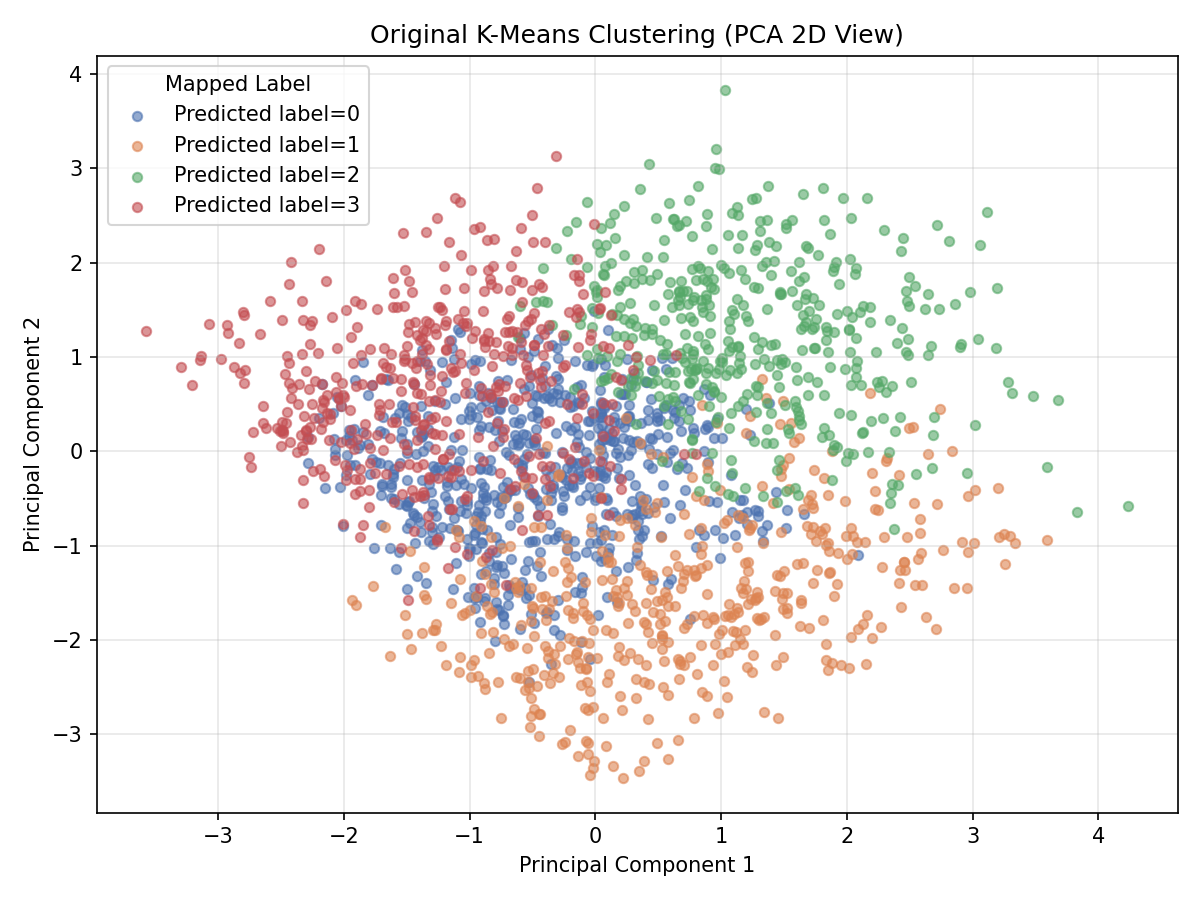
\includegraphics[width=0.48\textwidth]{pics/section5-1.png}
    \hfill
    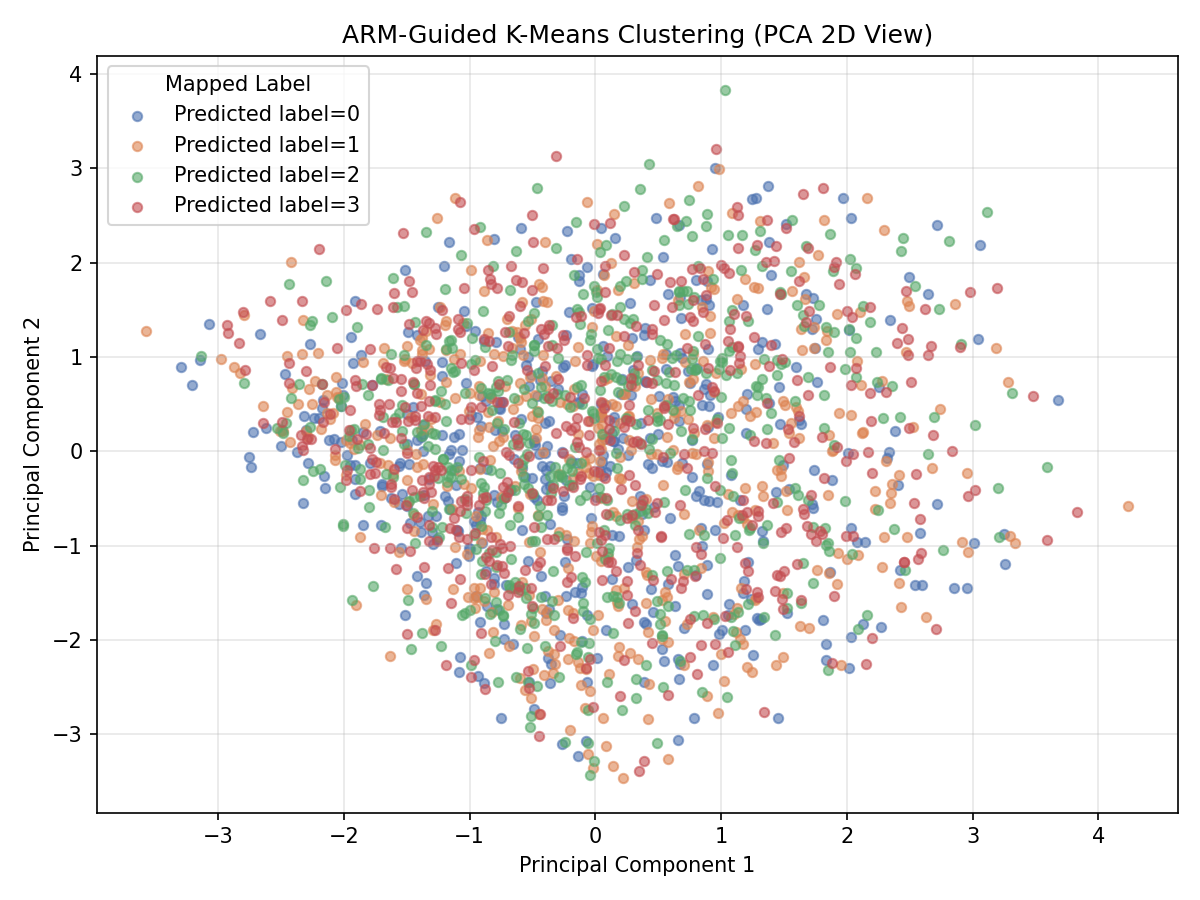
\includegraphics[width=0.48\textwidth]{pics/section5-2.png}
    \caption{Original K-means (left) and ARM-guided K-means (right), visualized in the same 2D PCA space.}
\end{figure}

One limitation of this visualization is that PCA only shows a two-dimensional projection of the original
standardized feature space. The ARM-guided method actually clusters in the full weighted feature space, so its
separation may not look cleaner in this 2D plot even when the quantitative performance is much better. Therefore,
the PCA figure should be used as a qualitative illustration, while the performance table is the main evidence for
comparing the two clustering methods.

% ---- Ablation Study ----
\subsection*{Ablation Study}

The ablation study shows that using only one ARM metric is not enough. Support alone favors common patterns,
confidence alone favors reliable rules, and lift alone favors surprising associations. Combining all three gives
a more balanced weight because a useful feature should be frequent enough, predictive enough, and more informative
than chance.

\begin{table}[H]
    \centering
    \begin{tabular}{@{}lcccc@{}}
        \toprule
        \textbf{Weight Variant} & \textbf{Accuracy} & \textbf{Precision} & \textbf{Recall} & \textbf{F1-score} \\ \midrule
        No weighting (baseline K-means)          & 0.2962 & 0.2959 & 0.2962 & 0.2941 \\
        Support only                              & 0.4760 & 0.4523 & 0.4760 & 0.4318 \\
        Confidence only                           & 0.6100 & 0.5825 & 0.6100 & 0.5884 \\
        Lift only                                 & 0.6221 & 0.5939 & 0.6221 & 0.5955 \\
        Support $\times$ Confidence $\times$ Lift & \textbf{0.7509} & \textbf{0.7555} & \textbf{0.7509} & \textbf{0.7522} \\ \bottomrule
    \end{tabular}
    \caption{Ablation study: effect of different ARM weight formulas (averaged over 5 seeds).}
\end{table}


\end{document}
